\documentclass[11pt]{article}
\usepackage{amsmath}
\usepackage{graphicx}
\usepackage[margin=1in]{geometry}
\usepackage{float}


\title{
  CS 4993-049
  Final Report 
}
\author{
  Geethan Sundaram
}
\date{
  Dec 17, 2024
}

\begin{document}
\maketitle


\section{Introduction}

This report serves as documentation of the research conducted and the system built and configured for the Fall 2024 semester under the guidance and investigation of Professor Hyojoon (Joon) Kim and Ph.D. student Di Zhu at the University of Virginia.

This report will document my work and understanding throughout the semester, including the assembly and functionality of the system and my understanding of the simulation + emulation codebase of Lightning: MIT's Reconfigurable Photonic SmartNIC.

\section{Components}

These are all the relevant components that make up the system:

\begin{table}[H]
\centering
\renewcommand{\arraystretch}{1.5}
\setlength{\tabcolsep}{6pt} % Adjust cell padding
\begin{tabular}{|p{0.15\textwidth}|p{0.4\textwidth}|p{0.2\textwidth}|p{0.2\textwidth}|}
\hline
\textbf{Component} & \textbf{Description} & \textbf{Part} & \textbf{Manufacturer} \\ \hline
Optical Table & Holds the entire system. & T36H & Thorlabs \\ \hline
Laser Diode & Provides the laser/light source to be used for optical computations. & CLD1010LP, LPS-PM1550-FC & Thorlabs \\ \hline
Modulator & Modulates light amplitudes using input electrical voltages. & LNA2322 & Thorlabs \\ \hline
Photodetector & Converts modulated light to voltage; performs calculations in vector scenarios. & RXM15EF & Thorlabs \\ \hline
RF Amplifier & Amplifies voltage for ADC/DAC connections to photodetectors and modulators. & LMH5401EVM & Texas Instruments \\ \hline
Fiber Polarization Controller & Adjusts polarization state of light to stabilize fiber connections. & FPC031 & Thorlabs \\ \hline
FPGA (Field Programmable Gate Array) & Generates signals for deep learning inferences; integrates ADC/DAC for signal conversion. & EK-U1-ZCU111-G & AMD \\ \hline
\end{tabular}
\caption{Main Components}
\label{table:components}
\end{table}


\begin{table}[H]
\centering
\renewcommand{\arraystretch}{1.5}
\setlength{\tabcolsep}{6pt} % Adjust cell padding
\begin{tabular}{{|p{0.15\textwidth}|p{0.4\textwidth}|p{0.2\textwidth}|p{0.2\textwidth}|}}
\hline
\textbf{Component} & \textbf{Description} & \textbf{Part} & \textbf{Manufacturer} \\ \hline
Aluminum Clamp & Holds the photodetector, can be fixed onto to the SBE1 base via a screw. & ECM175 & Thorlabs \\ \hline
Base & Holds up the photodetector through connection to the ECM175 clamp above the optical table & SBE1 & Thorlabs \\ \hline
Clamping Fork & Fixes the SBE1 base to the table via a screw. & SCF1 & Thorlabs \\ \hline
\end{tabular}
\caption{Photodetector Supporting Parts}
\label{table:components}
\end{table}


\begin{table}[H]
\centering
\renewcommand{\arraystretch}{1.5}
\setlength{\tabcolsep}{6pt} % Adjust cell padding
\begin{tabular}{{|p{0.15\textwidth}|p{0.4\textwidth}|p{0.2\textwidth}|p{0.2\textwidth}|}}
\hline
\textbf{Component} & \textbf{Description} & \textbf{Part} & \textbf{Manufacturer} \\ \hline
Single Mode Patch Cable & Connects laser source to the first modulator (if not provided already). & P5-1550PMP-1 & Thorlabs \\ \hline
Polarization-Matching Patch Cable & Connects second modulator to the photodetector (if not provided already). & P5-SMF28Y-FC-1 & Thorlabs \\ \hline
Adapters & For connecting fibers between each pair of wires. & [Unknown] & Thorlabs \\ \hline
Modulator Supports & Keep the modulators embedded into the optical table. & 3D-Printed & MIT \\ \hline
\end{tabular}
\caption{Modulator Supporting Parts}
\label{table:components}
\end{table}


\begin{table}[H]
\centering
\renewcommand{\arraystretch}{1.5}
\setlength{\tabcolsep}{6pt} % Adjust cell padding
\begin{tabular}{{|p{0.15\textwidth}|p{0.4\textwidth}|p{0.2\textwidth}|p{0.2\textwidth}|}}
\hline
\textbf{Component} & \textbf{Description} & \textbf{Part} & \textbf{Manufacturer} \\ \hline
SMA Male-Male Cables & For all connections with RF amplifiers (from photodetector to ADC's, and DAC's to modulators). & ECM175 & Thorlabs \\ \hline
DC Power Supply & Provides a direct current (DC) to the RF amplifer. & SPS-3010 & Jesverty \\ \hline
Banana Plug to Alligator Clip Test Leads & Connects SPS-3010 DC power supply to RF amplifier. & E-LEADS-BTA-4 & SDTC Tech \\ \hline
1 Male to 2 Female Splitter & Splits voltage from DC Power Supply. & W21067 & WJSTN \\ \hline
\end{tabular}
\caption{RF Amplifier Supporting Parts}
\label{table:components}
\end{table}


\section{System Overview}

\begin{figure}[H]
    \centering
    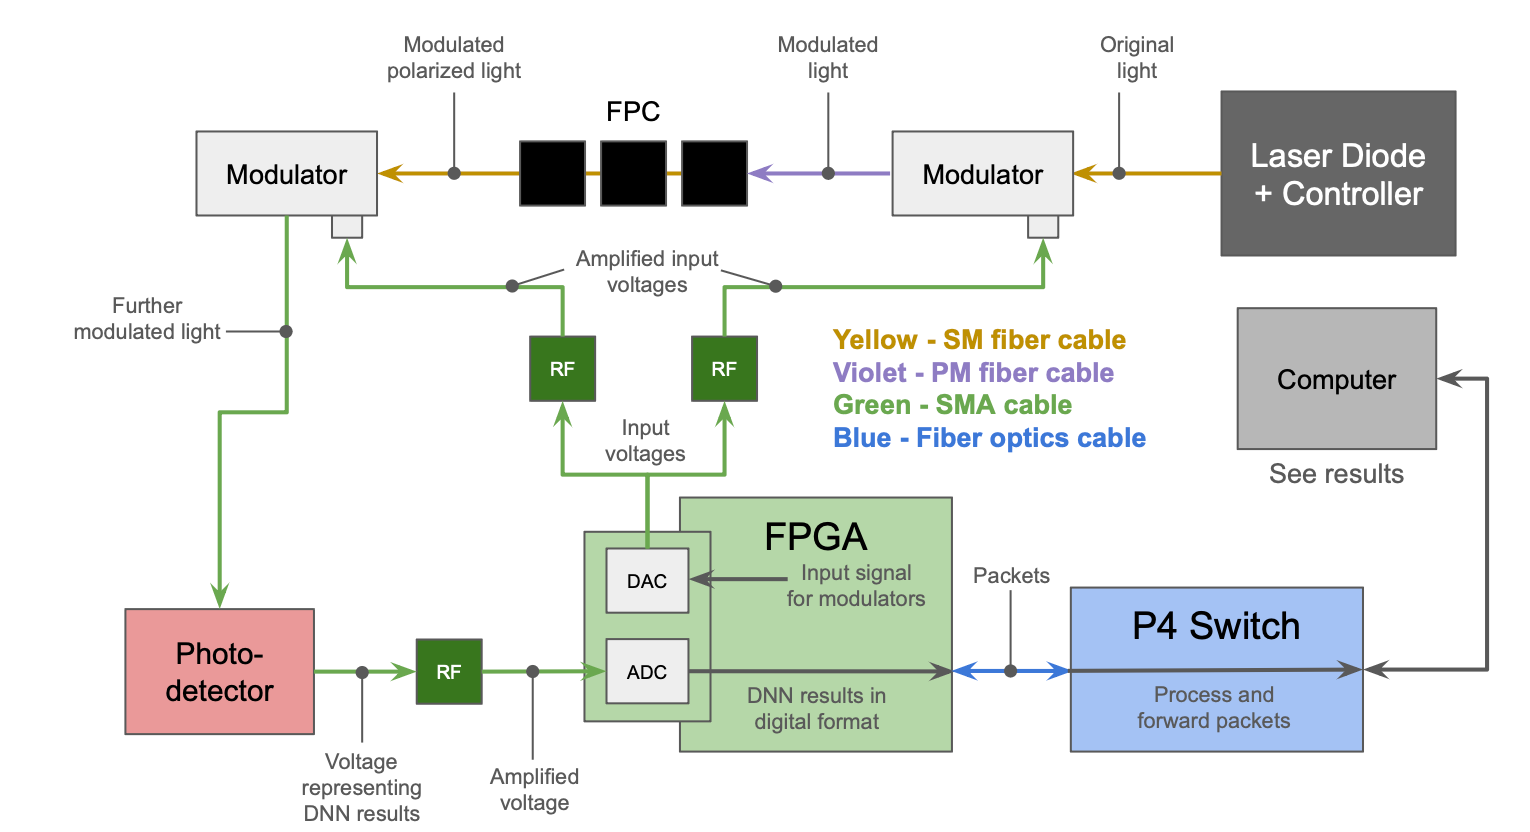
\includegraphics[width=1\linewidth]{image.png}
    \caption{System Diagram}
    \label{fig:enter-label}
\end{figure}

\subsection{Laser Diode}
The system begins with LP Pigtailed Laser Diodes (LPS-PM1550-FC) and a laser diode + temperature controller (CLD1010LP). The laser diode is responsible for converting the electricity it receives into light. This light is used for processing information and performing computation in photonic computing. 

The laser diode is mounted into the controller, allowing the functionality to control the intensity of the outputted light. This allows us to control the amount of light that we may use for our computations, with higher amounts of light corresponding to greater capabilities for carrying information, processing power, and more.

The rest of the laser diode is a PM cable. An important distinction is understanding the difference between single mode (SM) fiber and polarization-maintaining (PM) fiber cables. SM fiber transmits only one mode of light, or in other words, only one path for the light to propagate through, where the light may be randomly polarized with waves that have different frequencies. PM cables, on the other hand, ensure that only one polarization of the inputted light, or a constant direction for the light's vector field, is propogated throughout the fiber. This leads to PM fiber having higher attenuation, or a reduction in the light's power.

\subsection{First Modulation}

Each modulator (LNA2322) contains a PM fiber cable to take in an inputted light and a SM fiber cable to output the resultant light. The PM fiber of the laser diode connects to an adapter that connects to the first modulator's PM input fiber. The purpose of the adapter is to connect the fibers between the two cables, allowing light to be transmitted between them.

The modulator receives its input voltage from the FPGA (EK-U1-ZCU111-G). The modulator takes in the input voltage and adjusts its amplitude, or its intensity. This is done by taking in the modulator's input voltage, and essentially multiplying it with the light's amplitude to produce a de-amplified light. It then outputs this through its SM fiber cable, which connects to an adapter that connects to another SM fiber cable. 

It should be known that the modulators do not come with supports, and there do not exist any supports for purchase for the modulators from the manufacturers. However, the supports are not complicated to design via computer-aided design (CAD). Additionally, Lightning provides $.stl$ files for modulator supports that are ready to be 3D printed.

\subsection{Fiber Polarization}

The SM fiber cable is inserted within a Fiber Polarization Controller (FPC031). The FPC allows for adjusting the polarization of the light within the SM fiber that is inserted within it, which will be obtained from the output of the first modulator. 

The FPC contains three paddles: a quarter-wave plate, a half-wave plate, and a quarter-wave plate in that order. The first quarter-wave plate is responsible for transforming the polarization state of the input light to be linear. The half-wave plate rotates the polarization state of the input. Finally, the second-quarter wave plate transforms the linear polarization stage back into an output arbitrary output state to travel through the fiber. 

The purpose of the FPC in the system is due to the output cable of the first modulator being SM fiber and the input cable of the second modulator being PM fiber. The FPC adjusts the polarization of the SM cable accordingly to ensure that when the light enters the PM cable, there is no change in polarization and the de-amplified light is correctly transmitted between the two modulators. To put it shortly, the FPC ensures consistency in terms of the light's polarization as it enters different types of fibers.

\subsection{Second Modulation}

Following the adjustment of the polarization, the SM fiber connects to an adapter that connects to the PM fiber cable that is attached to the the second modulator and responsible for inputting light.

The same process as the first modulator occurs, where the light is multiplied by the input voltage of the modulator. The resulting output light can actually be represented as photonic multiplication. 
\begin{itemize}
  \item In the first modulator, we are multiplying the amplitude by the first input voltage, a - $(a \times L)$
  \item In the second modulator, we are multiplying that product by the second input voltage, b - $(b \times (a \times L))$
\end{itemize}
  Due to associativity, in the end, we are essentially multiplying the light by the product of all the input voltages - $((b \times a) \times L)$.

  This double modulated light is then transmitted via SM fiber to the photodetector.

\subsection{Photodetector}

The photodetector (RXM15EF) takes in the double modulated light from the second modulator and converts it into voltage.

The photodetector must be fixed to the table, which will require a base and a clamping fork, which was the SBE1 base and the SCF1 fork. Optionally, we may include a post that would be attached over the base if we wish to elevate the photodetector a certain distance over the optical table. The photodetector comes with a clamp (ECM175), which would be attached to the post or base, depending on whether the post is used or not.

Because of the photonic multiplication of input voltages, the voltage produced by the photodetector is equivalent to the product of these input voltages.

\begin{figure}[H]
    \centering
    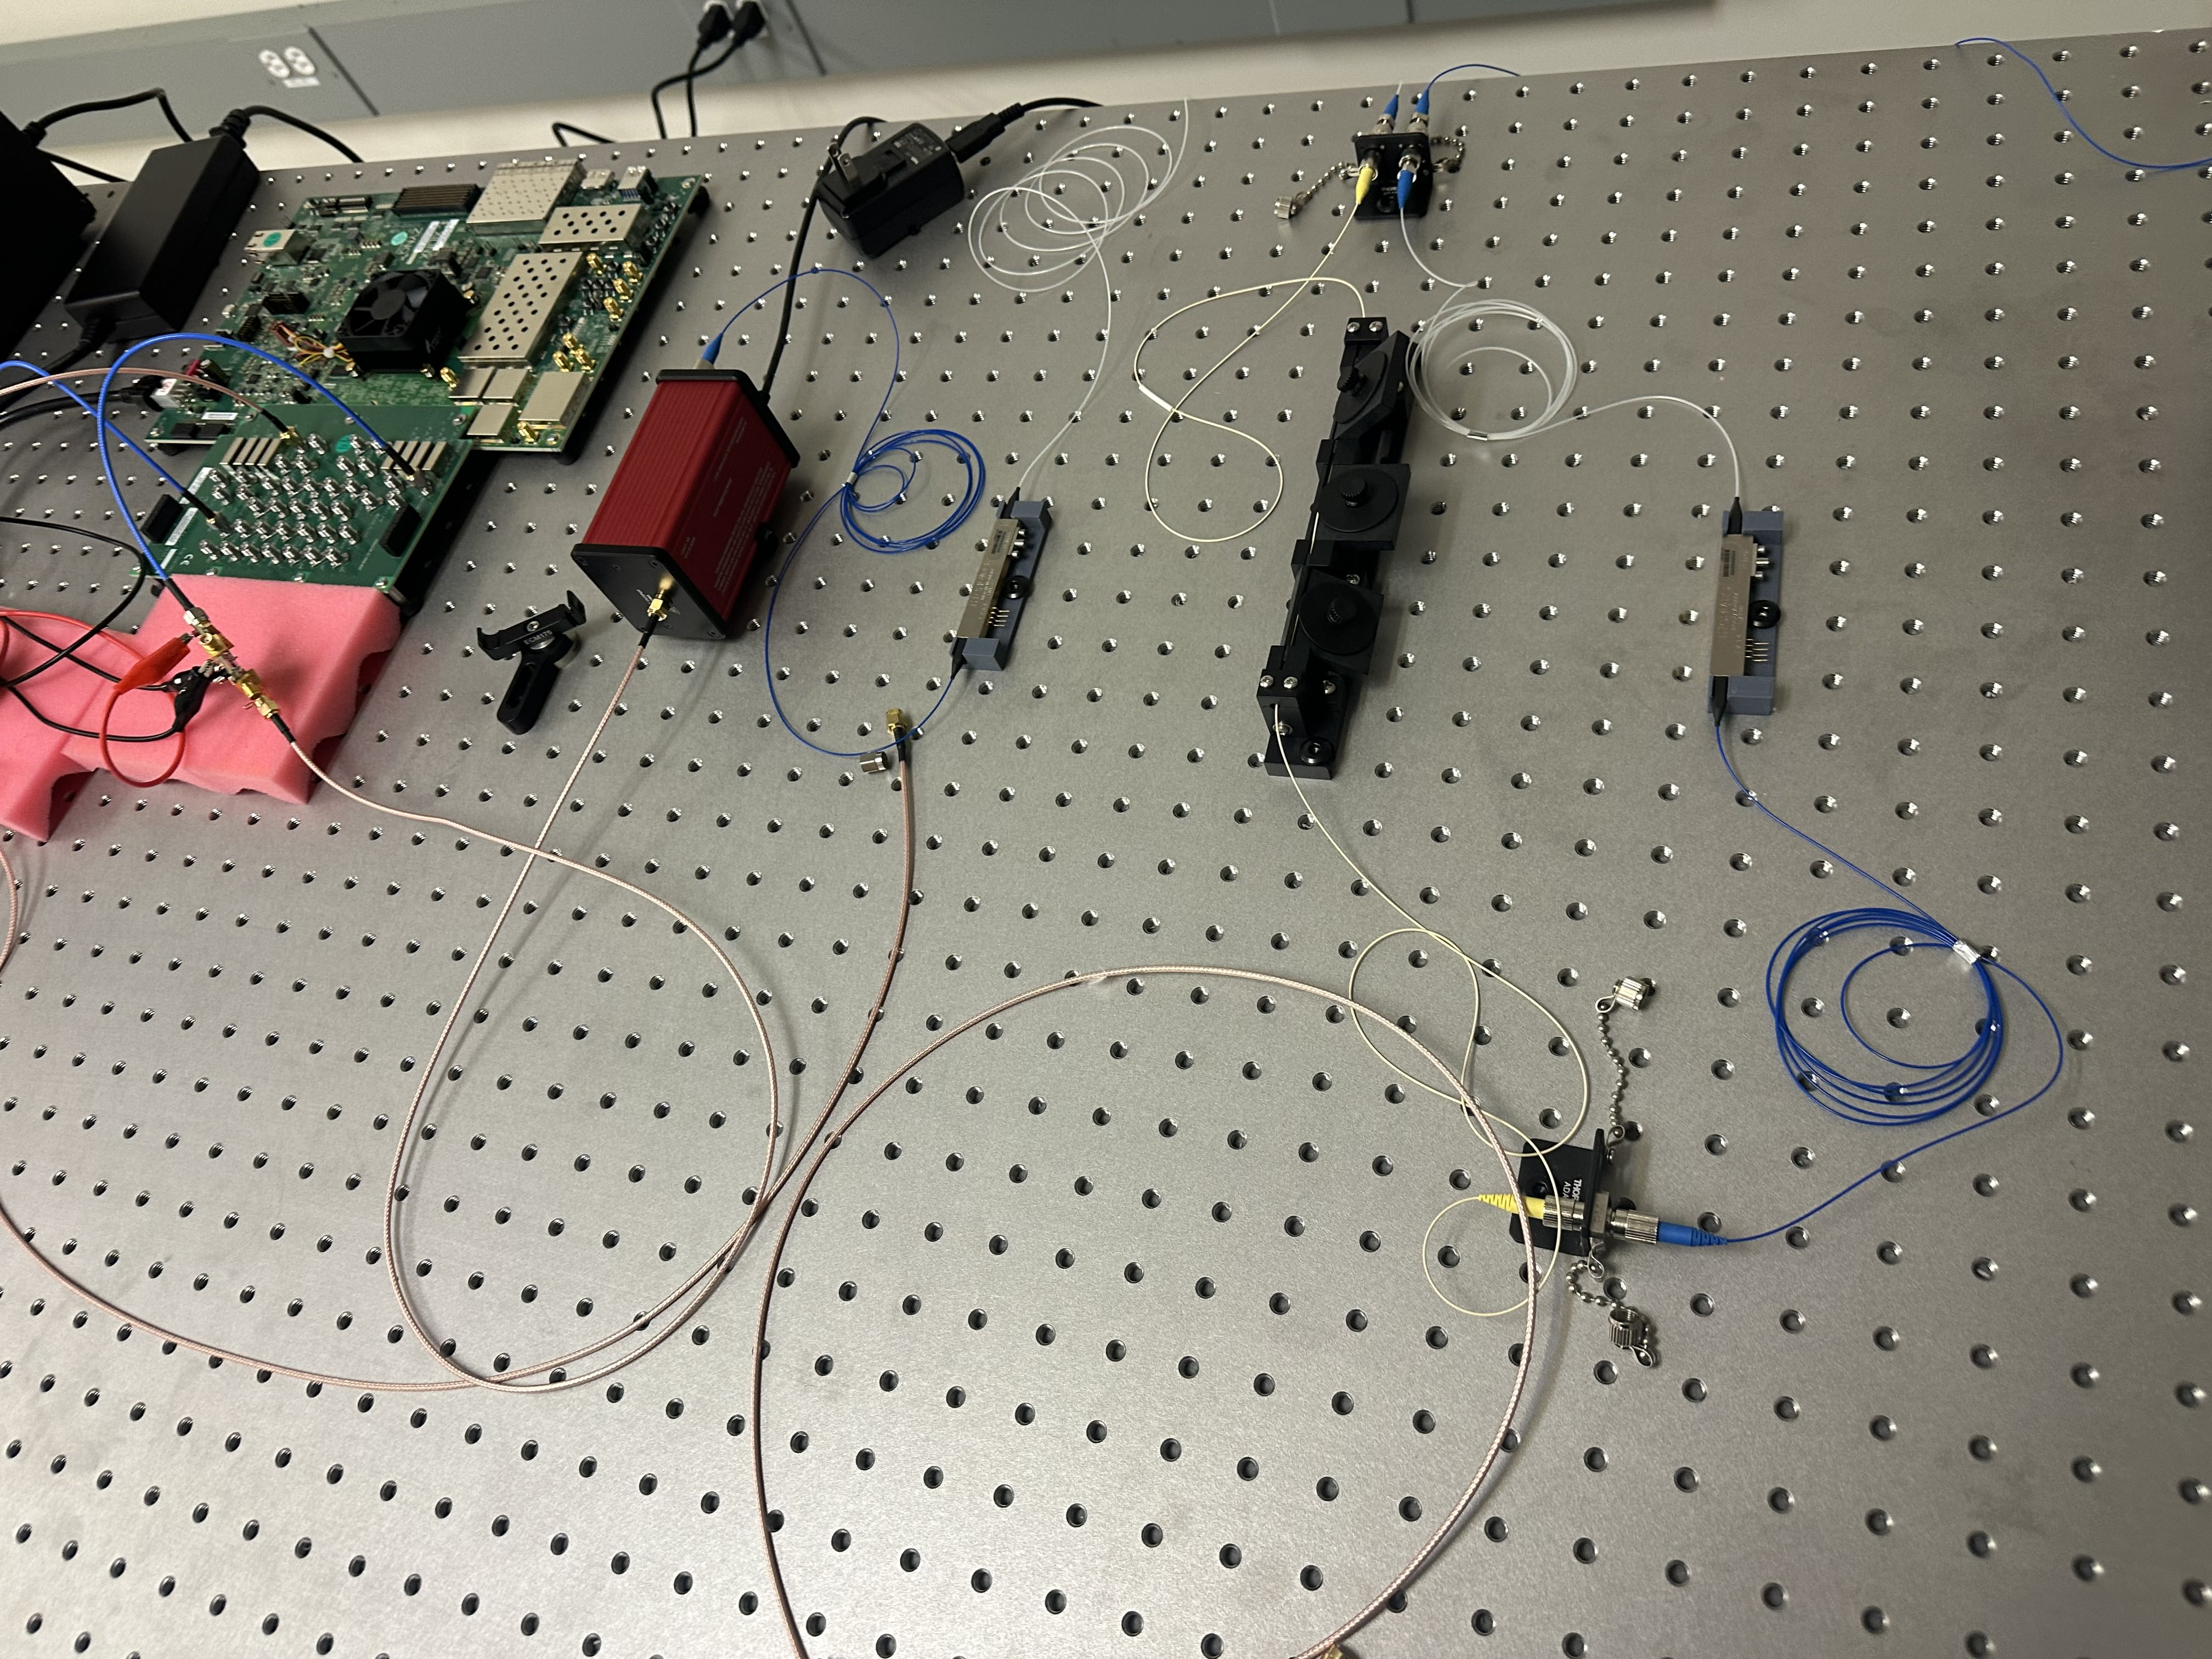
\includegraphics[width=0.5\linewidth]{modsandpd.jpg}
    \caption{Set up of Modulators, FPC, and Photodetector}
    \label{fig:enter-label}
\end{figure}

\subsection{FPGA}

The outputted voltage from the photodetector is sent to the FPGA (EK-U1-ZCU111-G). The FPGA is responsible for controlling the optical system and processing the computations that it performs. 

The FPGA has ADC's (analog-to-digital converters) and DAC's (digital-to-analog converters). The rest of the system uses light and voltage, which which are analog signals, while the FGPA works with digital (binary) signals. Therefore, these converters are necessary to ensure that all necessary information is being transmitted throughout the system and being understood by each section.

The FPGA is designed to be programmable for the purpose of helping in configuring the overall system and successfully transmitting data. This can be acheived via Verilog, a hardware description language (HDL) for digital circuits. We can program the input voltages that we desire to send to our modulators by programming the FPGA, which will send over the correct voltages to each modulator, resulting in the appropriate calculations in the analog domain due to those voltages. Since the FPGA only understands binary data and the modulator must take in a voltage, the DAC is necessary to convert the digital signal from the FGPA into an analog voltage for the modulator to understand and take in as an input.

The light from the laser diode travels throughout the entire system, carrying all the information of the calculations that took place, and after departing the photodetector, reaches the FGPA. The light is an analog signal, so it cannot be understood by the FPGA. The ADC solves this issue by converting the light into a digital format that the FPGA is able to understand. The FPGA then sends this information to the P4 switch, which will be responsible for processing the packets from the FPGA based on our specifications and needs. Unfortunately, the FPGA has not been configured yet in our system, but if it were to exist, that will be its purpose.

\begin{figure}[H]
    \centering
    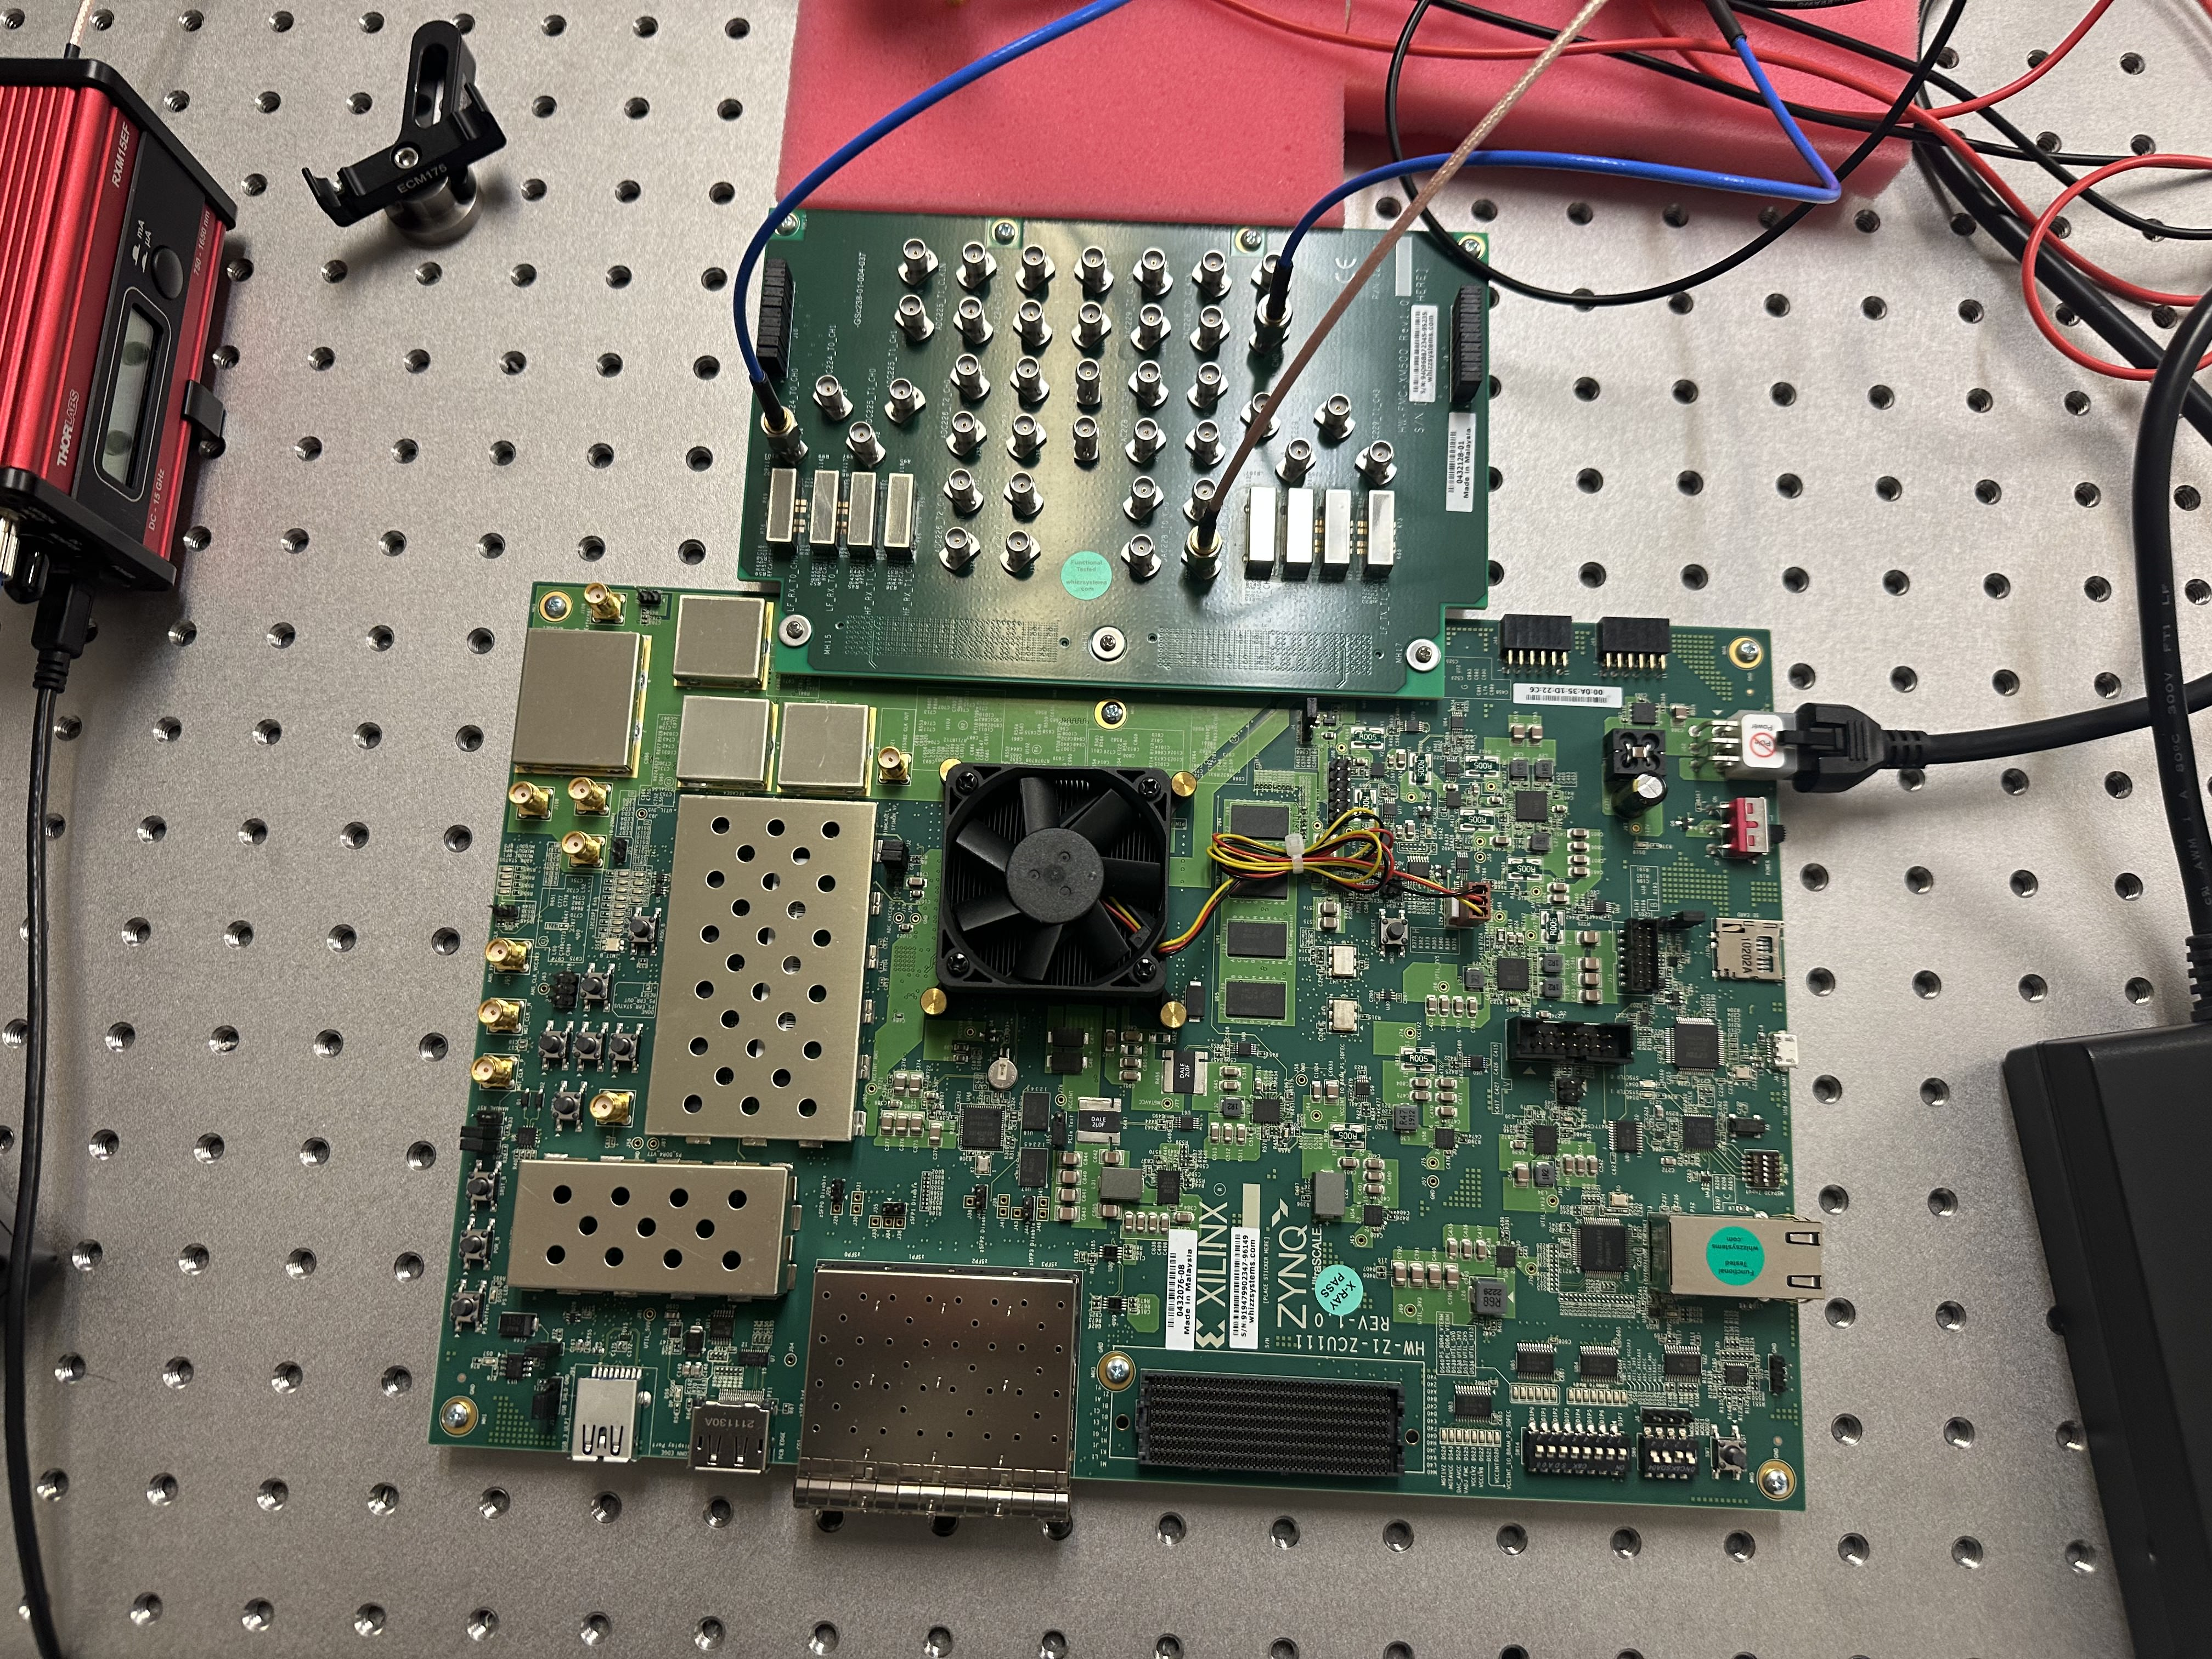
\includegraphics[width=0.5\linewidth]{fpga.jpg}
    \caption{FPGA with ADC's and DAC's}
    \label{fig:enter-label}
\end{figure}

\subsection{RF Amplifier}

The RF amplifiers (LMH5401EVM) are placed between the photodetector and the ADC and between each DAC and modulator. The outputted voltage from the DAC of the FPGA is insufficient for the modulator. To compensate for this lack of voltage, RF amplifiers amplify the voltage from the DAC before it reaches the modulator, ensuring a larger voltage range capable of matching the modulator's half-wave voltage. The photodetector's voltage is also insufficient for the ADC, requiring an additional RF amplifier to add additional voltage to the photodetector's output voltage to be sufficient (1.2 V CMV).

The RF amplifiers are powered by direct current (DC) and require DC power supplies to enable them to function.

\begin{figure}[H]
    \centering
    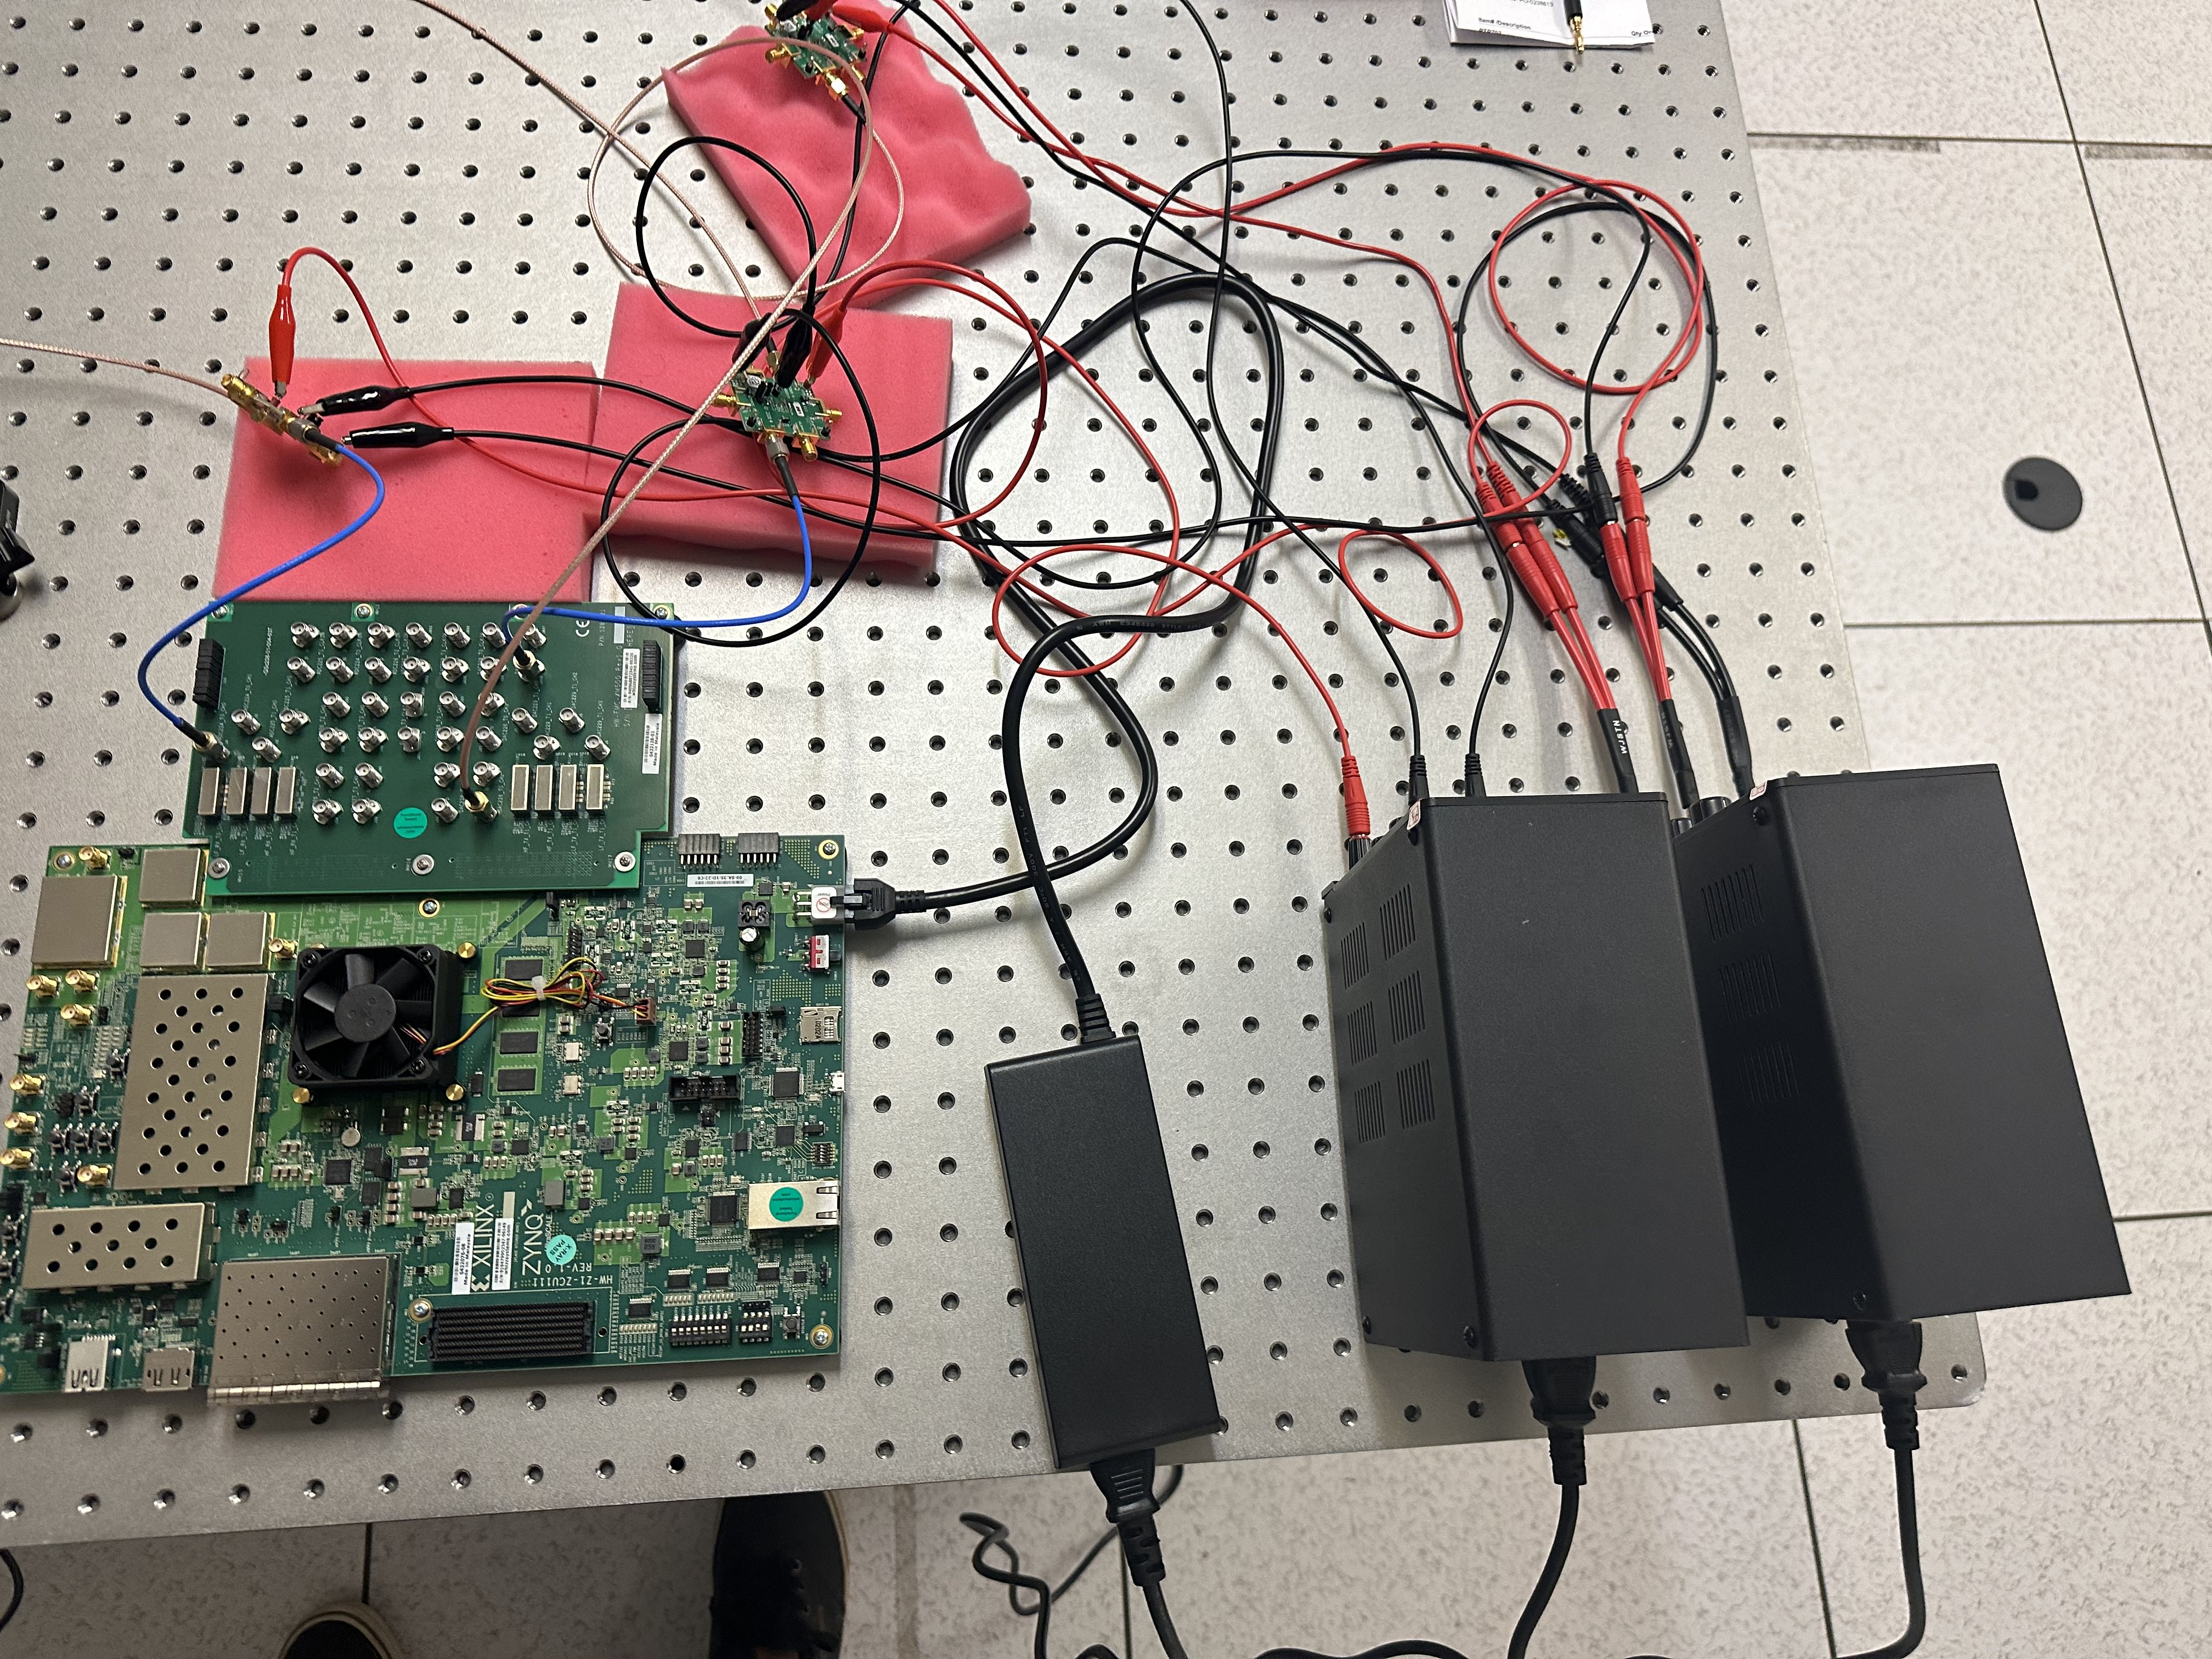
\includegraphics[width=0.5\linewidth]{rfamplifiers.jpg}
    \caption{RF Amplifiers with their power supplies}
    \label{fig:enter-label}
\end{figure}

\subsection{Running the System}

To turn the light on, first flip the switch on the back of the laser diode controller:

\begin{figure}[H]
    \centering
    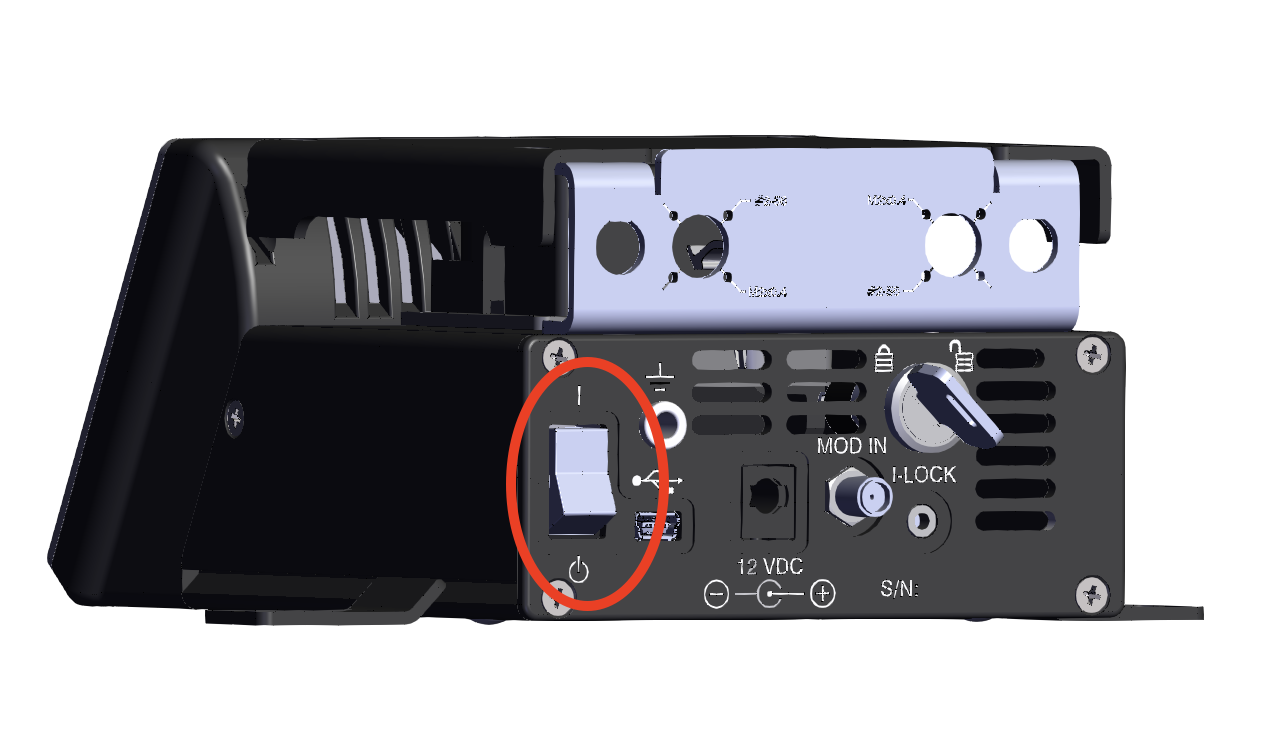
\includegraphics[width=0.5\linewidth]{diodeswitch.png}
    \label{fig:enter-label}
\end{figure}

This turns on the controller, which allows us to turn on the laser and provide necessary adjustments. The controller will display the following screen on its touch panel:

\begin{figure}[H]
    \centering
    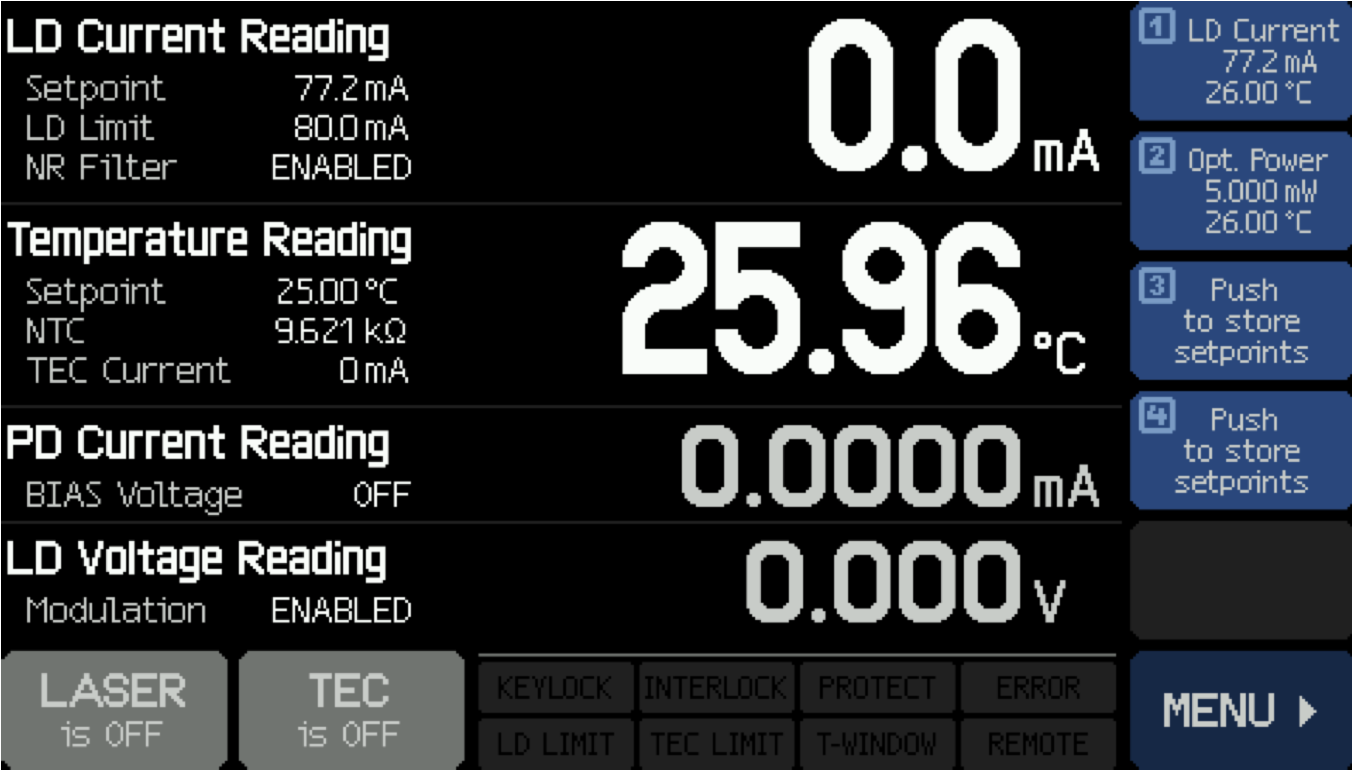
\includegraphics[width=0.5\linewidth]{laseroff.png}
    \label{fig:enter-label}
\end{figure}

The laser should be in Constant Current (CC) mode, as that is recommended for modulation of the light. You can ensure this is the case by seeing the units of the laser on the display being $mA$ instead of $mW$.

Turn on the laser by toggling the button on the touch screen that reads "\textit{LASER is OFF}." If it is green and says "\textit{LASER is ON}" then the laser has been successfully activated.

\begin{figure}[H]
    \centering
    
\includegraphics[width=0.1\linewidth]{laseron.png}
    \label{fig:enter-label}
\end{figure}

To adjust the current of the light, press the current display, which is the large number at the top. This will provide \textbf{+} and \textbf{-} buttons on the right-most side of the touch screen to increase or decrease the digit of the laser's current that a cursor is currently on. To shift the cursor to adjust a another digit, press the $\Leftarrow$ and $\Rightarrow$ buttons. After adjusting the value, in order to save these changes press the green \textit{DONE} button to finish. If you do not wish to save your changes, press the red \textit{ESC} button.

\begin{figure}[H]
    \centering
    
\includegraphics[width=0.1\linewidth]{buttons.png}
    \label{fig:enter-label}
\end{figure}

When the light exits the first modulator and goes through the FPC, adjust the three plates accordingly to adjust the polarization of the light so that the information carried in the light remains consistent throughout the light's transmission through different cable fibers.

Ensure that the photodetector is on by flipping the power switch on its left end:

\begin{figure}[H]
    \centering
    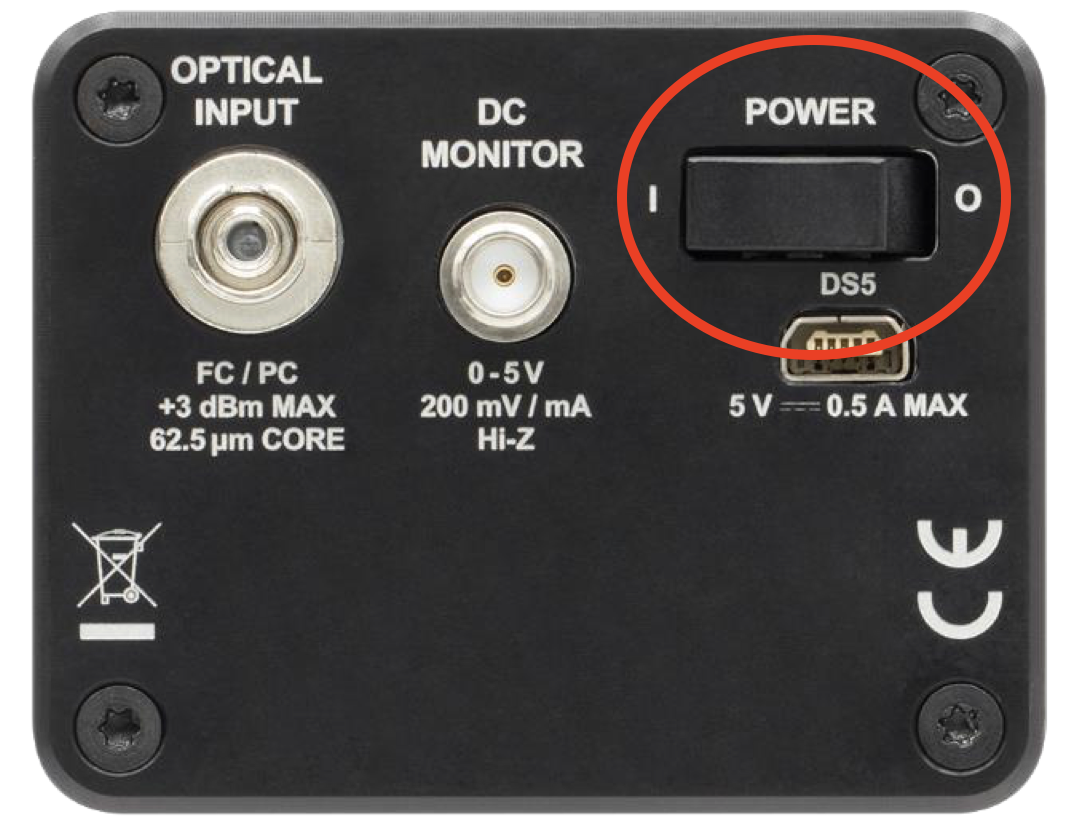
\includegraphics[width=0.5\linewidth]{pdonoff.png}
    \label{fig:enter-label}
\end{figure}

When the light exits the second modulator and enters the photodetector, the photodetector provides readings on its display of the photocurrent of the light, with the option to toggle between $\mu A$ (microampere) or $mA$ (milliampere) using a button next to the display.

\section{Lightning Simulation}

The purpose of the simulation is to see how Lightning compares to other processors in terms of speed and energy efficiency.

\subsection{Context}

The simulation aims to compare Lightning with an Nvidia A100 GPU, an A100X DPU, and a Brainwave SmartNIC.

In the simulation, there are 10 pickle files with their own identification pickle number, each containing their own unique schedule of machine learning inferences for the simulator to go through.

In the simulation, a DNN inference is referred to as a request. A layer of the DNN inference is referred to as a job. 

\subsection{Process}
The process of the simulation is as follows:

\begin{enumerate}
    \item \textbf{bash run.sh} - Runs 4 simulations in parallel for each pickle file, each with one of the following processors: Lightning, Nvidia A100 GPU, A100X DPU, and Brainwave SmartNIC.
    \begin{description}
        \item[sim.py] Runs a simulation
        \begin{enumerate}
            \item Parses command line arguments to get necessary parameters for processor, network speed, pickle number, final request, and more.
            \item Simulates the scheduling and processing of several DNN model requests on the inputted processor.
            \item Creates and configures a simulator instance to handle several requests with different arrive times and request rates based on network speed.
            \item The simulator processes all the requests and all the jobs within it.
            \item Calculates the average request time for each model after simulation is done.
            \item Retrieves and stores the count of the requests over time (how many requests were active during each point in time)
            
        \end{enumerate}
    \end{description}

    \item \textbf{bash csv\_gen.sh} - Converts the simulator's trial outputs to a readable CSV format
    \begin{description}
        \item[trial\_to\_csv.py] Converts trial log to CSV
        \begin{enumerate}
            \item Parses command line arguments to get necessary parameters for processor, network speed, pickle number, number of requests, and more.
            \item When average request completion time, total runtime, and count of active requests over time are all found, total runtime with average completion time per model and active requests over time are returned as strings
            \item If they are all not found, a string is stored with the partial data that is available
            \item The results are outputted into a CSV file using the strings
        \end{enumerate}
    \end{description}

    \item \textbf{bash final\_gen.sh} - Generates a TSV-formatted file containing the average runtimes of each DNN model with each processor
    \begin{description}
        \item[read\_csv.py] Processes runtime data for the DNNs on each processor and stores the results into a TSV-formatted file
        \begin{enumerate}
            \item Parses command line arguments to get necessary parameters for cores, batch size, and type of scheduling.
            \item For each pickle file, the corresponding CSV file is parsed
            \item For that pickle number, it finds ratios for other processors against Lightning for each model, tracking the maximum ratio
            \item Returns a string containing formatted runtimes and ratios
            \item The results are outputted into a TSV-format using the string 
        \end{enumerate}
    \end{description}

    \item \textbf{congestion\_plot.py} - Plots the active requests over time for each processor for the given network speed

    \begin{figure}[H]
    \centering
    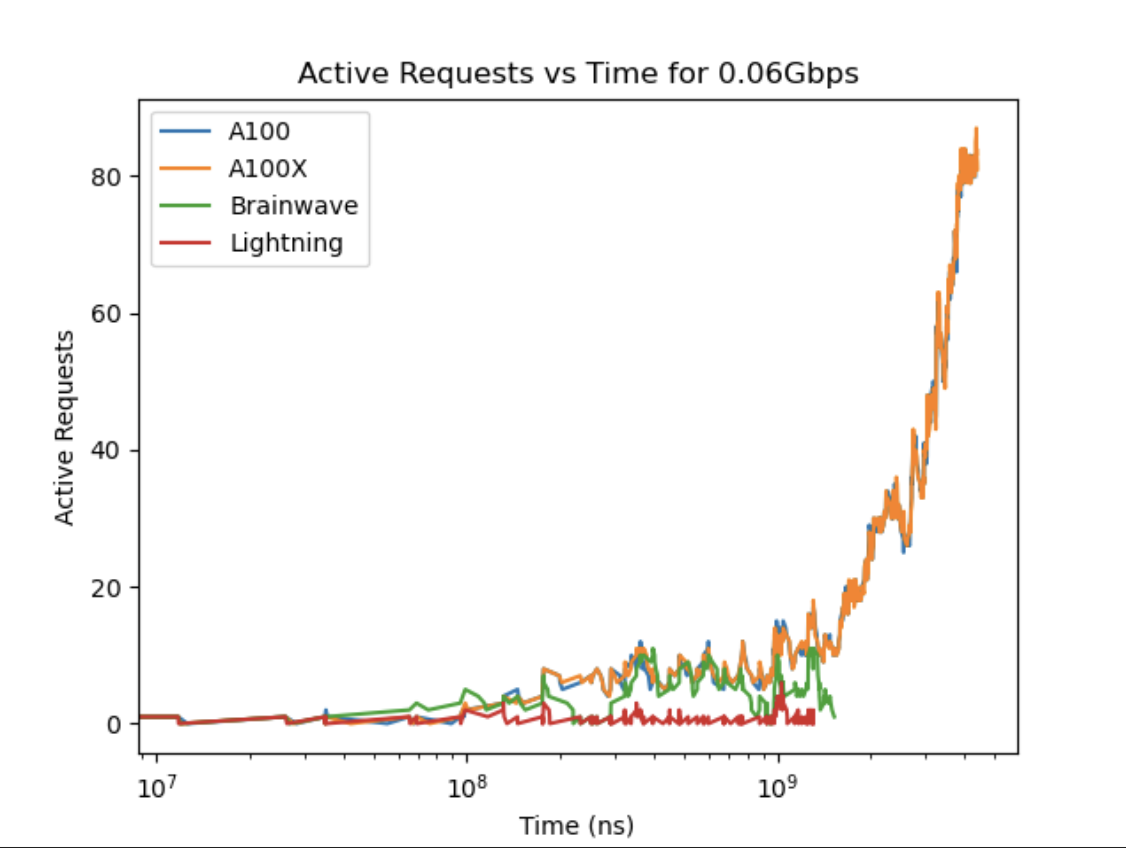
\includegraphics[scale=.75]{congestion.png}
    \caption{Congestion Plot of Active Requests vs. Time}
    \label{fig:enter-label}
\end{figure}

    Note that Lightning remains the lowest curve, showing the least amount of requests marked during each noted point in time, indicating the least amount of request congestion overall.

\end{enumerate}

\section{Lightning Emulation}

This will be a very short section where I describe the emulation and its purpose.

The emulation runs emulations for four convolutional neural network (CNN) architectures: AlexNet, VGG-11, VGG-16, and VGG-19.

For each model, the emulation defines it in three different forms:
\begin{enumerate}
    \item \textbf{32-bit} - This represents the model with the highest possible precision, as it typically would be without any real-world interruption or inconsistencies. The model utilizes 32-bit inputs, which enables high precision due to the large amount of bits used to represent the inputs.
    \item \textbf{8-bit} - The inputs and activations from the 32-bit model are converted into 8-bit integers, which slightly reduces precision but improves computational speed, memory efficiency, and energy efficiency. Input and intermediate tensors are converted into an 8-bit range and rounded to integer precision. Bias values are scaled to ensure that the new activations still align with the biases in the model at the same scaling.
    \item \textbf{8-bit w/ noise} - Gaussian noise is added to the activations of the 8-bit model using a normal distribution. This represents the model in a real-world setting, where the state of the environment cannot be ideal. This robustness is representative of Lightning when running an inference.

The purpose of the emulation is to compare Lightning to these more ideal versions of the same models, and measure that the loss in precision is not substantial enough due to the lower bits' inability to represent the full range of 32 bits and the noise emerging from a non-ideal environment.

\end{enumerate}

\section{Conclusion}

We have delved into the components and organization of the current system as a whole, as well as touched on Lightning's simulation and emulation, which were all the pivotal focus points of this research position.

To conclude this report, I would like to pose some questions and concerns to consider and look into for the future for better understanding:

\begin{enumerate}
    \item What is the technicality behind the polarization of light? How exactly does the FPC ensure consistency of information through the changing polarization?
    \item What programs are necessary for the FPGA and how will they be implemented? This includes both the input voltages it provides for the modulators as well as its ability to transfer the photodetector readings to the P4 switch.
    \item What is the significance of each DAC and ADC, since there are several of them with seemingly different purposes?
    \item What is the reason for there existing  varying implementations of the simulation due to varying factors like batch size and scheduling, but the code only simulating one value for them? \textbf{EX: only preemptive scheduling is used for all processor simulations but non-preemptive is also implemented.}
    \item Why does the emulation represent Lightning as 8-bit rather than 32-bit? Why is this loss in precision present and necessary?
    
\end{enumerate}

\end{document}